\documentclass[12pt,letterpaper]{exam}
\usepackage[lmargin=1in,rmargin=1in,tmargin=1in,bmargin=1in]{geometry}
\usepackage{../style/exams}

% -------------------
% Course & Exam Information
% -------------------
\newcommand{\course}{MAT 101: Exam 2}
\newcommand{\term}{Spring -- 2022}
\newcommand{\examdate}{04/14/2022}
\newcommand{\timelimit}{85 Minutes}

\setbool{hideans}{true} % Student: True; Instructor: False

% -------------------
% Content
% -------------------
\begin{document}

\examtitle
\instructions{Write your name on the appropriate line on the exam cover sheet. This exam contains \numpages\ pages (including this cover page) and \numquestions\ questions. Check that you have every page of the exam. Answer the questions in the spaces provided on the question sheets. Be sure to answer every part of each question and show all your work.} 
\scores
%\bottomline
\newpage

% ---------
% Questions
% ---------
\begin{questions}

% Question 1
\newpage
\question[10] Sketch the quadratic function $f(x)= 8 - \left( x - \dfrac{13}{2} \right)^2$ on the plot below. Your sketch should include the vertex and axis of symmetry---being placed as accurately as possible. 
	\[
	\fbox{
	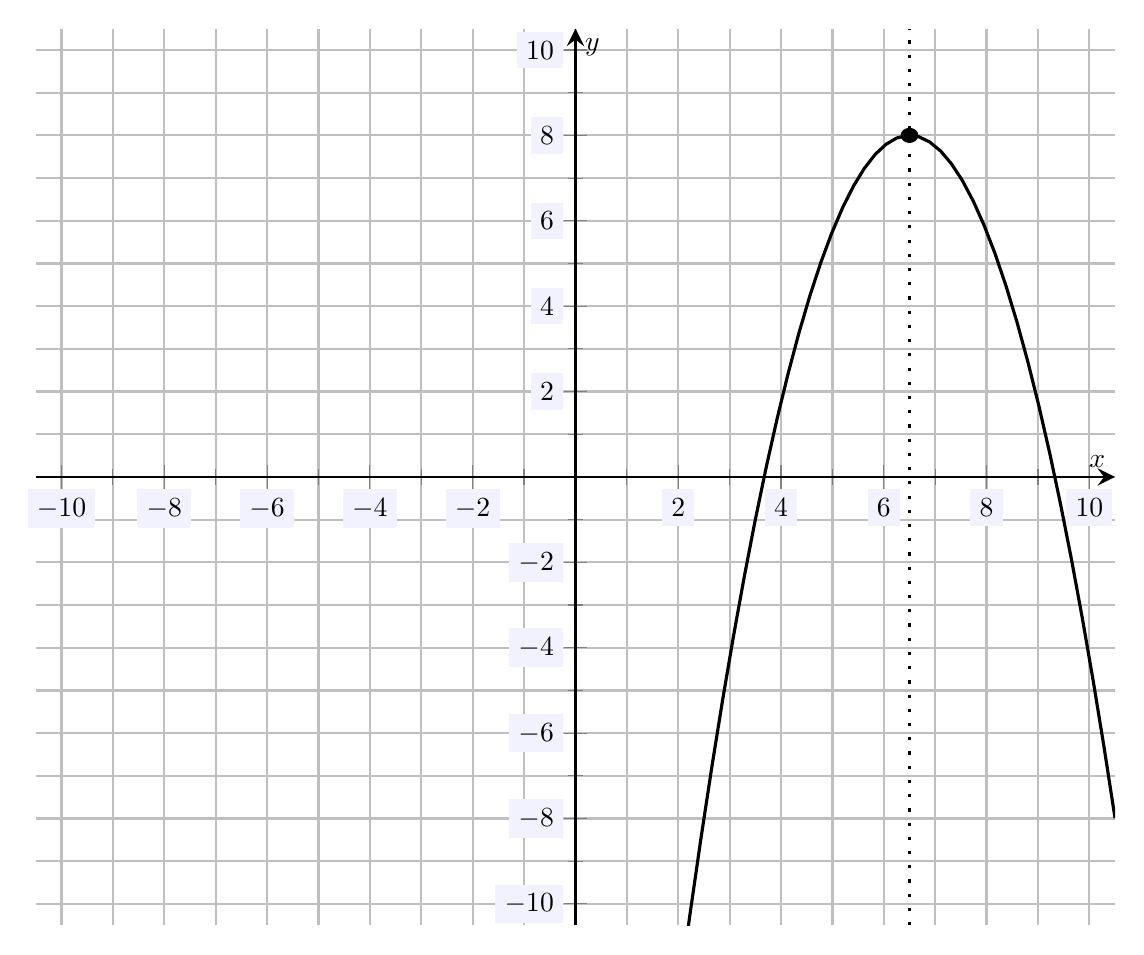
\begin{tikzpicture}[scale=2,every node/.style={scale=0.5}]
	\begin{axis}[
	grid=both,
	axis lines=middle,
	ticklabel style={fill=blue!5!white},
	xmin= -10.5, xmax=10.5,
	ymin= -10.5, ymax=10.5,
	xtick={-10,-8,-6,-4,-2,0,2,4,6,8,10},
	ytick={-10,-8,-6,-4,-2,0,2,4,6,8,10},
	minor tick = {-10,-9,...,10},
	xlabel=\(x\),ylabel=\(y\),
	]
	\draw[fill=black] (13/2,8) circle (0.15);
	\draw[line width=0.02cm,dotted] (13/2,-10.5) -- (13/2,10.5);
	\addplot[line width= 0.02cm,samples=100,domain= -10.5:10.5] ({x},{8 - (x- 13/2)^2}); 
	\end{axis}
	\end{tikzpicture}
	}
	\] \pspace

{\itshape We have $f(x)= 8 - \left( x - \dfrac{13}{2} \right)^2= - \left( x - \dfrac{13}{2} \right)^2 + 8$. Therefore, $f(x)$ is in vertex form, i.e. the form $f(x)= a(x - p)^2 + q$, where $(p, q)$ is the vertex. We then know that the vertex of $f(x)$ is $(-\frac{13}{2}, 8)$ so that the axis of symmetry is $x= \frac{13}{2}$. Because $a= -1 < 0$, the parabola opens downwards. This gives the sketch above.}



% Question 2
\newpage
\question Consider the quadratic function $y= (x + 5)^2 + 6$.

\begin{parts}
\part[2] Identify $a$, $b$, and $c$ for this quadratic function. \pvspace{0.3cm}

{\itshape
	\[
	y= (x + 5)^2 + 6= (x^2 + 10x + 25) + 6= x^2 + 10x + 31
	\] \pspace
Therefore, $a= 1$, $b= 10$, $c= 31$.} \pvspace{0.9cm}

\part[2] Does this quadratic function open upwards or downwards? \pvspace{1.6cm}

{\itshape Because $a= 1 > 0$, the quadratic function opens upwards.} \pvspace{1.6cm}

\part[2] Is this quadratic function convex or concave? \pvspace{1.6cm}

{\itshape Because $a= 1 > 0$, the quadratic function is convex} \pvspace{1.6cm}

\part[2] What is the vertex of this quadratic function? What is the axis of symmetry? \pvspace{1cm}

{\itshape The quadratic function $y= (x + 5)^2 + 6$ is in vertex form, i.e. $y= a(x - p)^2 + q$, where $(p, q)$ is the vertex. Therefore, the vertex is $(-5, 6)$ and the axis of symmetry is $x= -5$.} \pvspace{1cm}

\part[2] Find the maximum and minimum values for $y$. \pvspace{1cm}

{\itshape Because the parabola opens upwards, there is no maximum value, i.e. it does not exist. The parabola has a minimum. Because the vertex is $(-5, 6)$, we know the minimum value is 6---the $y$-coordinate of the vertex.}
\end{parts}



% Question 3
\newpage
\question[10] Find the vertex form of the quadratic function $f(x)= -3x^2 + 12x - 7$. \pspace

{\itshape Completing the square, we have\dots
	\[
	\begin{aligned}
	f(x)&= -3x^2 + 12x - 7 \\
	&= -3 \left( x^2 - 4x + \dfrac{7}{3} \right) \\
	&= -3 \left( x^2 - 4x + 4 - 4 + \dfrac{7}{3} \right) \\
	&= -3 \left( (x^2 - 4x + 4) - \dfrac{12}{3} + \dfrac{7}{3} \right) \\
	&= -3 \left( (x - 2)^2 - \dfrac{5}{3} \right) \\
	&= -3(x - 2)^2 + 5
	\end{aligned}
	\] \pspace
Alternatively, we can use the `evaluation method':
	\[
	\begin{aligned}
	a&= -3 \\
	x&= -\dfrac{b}{2a}= -\dfrac{12}{2(-3)}= -\dfrac{12}{-6}= -(-2)= 2 \\
	f(2)&= -3(2^2) + 12(2) - 7= -3(4) + 12(2) - 7= -12 + 24 - 7= 5
	\end{aligned}
	\]
Therefore, the vertex form is $f(x)= -3(x - 2)^2 + 5$. 
}



% Question 4
\newpage
\question[10] Factor $x^2 + 16x - 80$ completely. \pspace

{\itshape
	\begin{table}[!ht]
	\centering
	\underline{\bfseries 80} \pvspace{0.2cm}
	\begin{tabular}{rr}
	$1 \cdot -80$ & $-79$ \\
	$-1 \cdot 80$ & $79$ \\
	$2 \cdot -40$ & $-38$ \\
	$-2 \cdot 40$ & $38$ \\
	$4 \cdot -20$ & $-16$ \\ \hline
	\multicolumn{1}{|r}{$-4 \cdot 20$} & \multicolumn{1}{r|}{$16$} \\ \hline
	$5 \cdot -16$ & $-11$ \\
	$-5 \cdot 16$ & $11$ \\
	$8 \cdot -10$ & $-2$ \\
	$-8 \cdot 10$ & $2$
	\end{tabular}
	\end{table}

Therefore,
	\[
	x^2 + 16x - 80= (x - 4)(x + 20)
	\] 
}



% Question 5
\newpage
\question[10] Factor $3x^2 - 9x - 120$ completely. \pspace

{\itshape First, observe that $3x^2 - 9x - 120= 3(x^2 - 3x - 40)$. Then\dots
	\begin{table}[!ht]
	\centering
	\underline{\bfseries 40} \pvspace{0.2cm}
	\begin{tabular}{rr}
	$1 \cdot -40$ & $-39$ \\
	$-1 \cdot 40$ & $39$ \\
	$2 \cdot -20$ & $-18$ \\
	$-2 \cdot 20$ & $18$ \\
	$4 \cdot -10$ & $-6$ \\
	$-4 \cdot 10$ & $6$ \\ \hline
	\multicolumn{1}{|r}{$5 \cdot -8$} & \multicolumn{1}{r|}{$-3$} \\ \hline
	$-5 \cdot 8$ & $3$ 
	\end{tabular}
	\end{table}

Therefore,
	\[
	3x^2 - 9x - 120= 3(x^2 - 3x - 40)= 3(x + 5)(x - 8)
	\] 
}



% Question 6
\newpage
\question Factor the following completely: \pspace

\begin{parts}
\part[5] $16x - 20x^2$ \pvspace{1cm}

{\itshape Observe, we can factor out $4x$:
	\[
	16x - 20x^2= 4x(4 - 5x)
	\]
} \pvspace{6.85cm}

\part[5] $49 - x^2$ \pvspace{1cm}

{\itshape Observe that this is a difference of perfect squares:
	\[
	49 - x^2= (7 - x)(7 + x)
	\]
}
\end{parts}



% Question 7
\newpage
\question[10] Factor $10x^2 + 43x - 35$ completely. 



% Question 8
\newpage
\question[10] Solve the following:
	\[
	5(6 - x)= \dfrac{4}{3}\,x + 30
	\] \pspace

	\[
	\begin{aligned}
	5(6 - x)&= \dfrac{4}{3}\,x + 30 \\[0.3cm]
	30 - 5x&= \dfrac{4}{3}\,x + 30 \\[0.3cm]
	-5x&= \dfrac{4}{3}\,x \\[0.3cm]
	-15x&= 4x \\[0.3cm]
	-19x&= 0 \\[0.3cm]
	x&= 0
	\end{aligned}
	\]



% Question 9
\newpage
\question[10] Solve the following:
	\[
	9= x(10 - x)
	\] \pspace

{\itshape
	\[
	\begin{aligned}
	9= x(10 - x) \\[0.3cm]
	9= 10x - x^2 \\[0.3cm]
	x^2 - 10x + 9= 0 \\[0.3cm]
	(x - 1)(x - 9)= 0
	\end{aligned}
	\] \pspace
But then either $x - 1=0$, so that $x= 1$, or $x - 9=0$, so that $x= 9$.}



% Question 10
\newpage
\question[10] Solve the following:
	\[
	6 - x= 12x + 7
	\] \pspace

	\[
	\begin{aligned}
	6 - x&= 12x + 7 \\[0.3cm]
	-1&= 13x \\[0.3cm]
	x&= -\dfrac{1}{13}
	\end{aligned}
	\] 



% Question 11
\newpage
\question[10] Solve the following:
	\[
	x(3x - 1)= x(x + 5)
	\] \pspace

{\itshape
	\[
	\begin{aligned}
	x(3x - 1)&= x(x + 5) \\[0.3cm]
	3x^2 - x&= x^2 + 5x \\[0.3cm]
	2x^2 - 6x&= 0 \\[0.3cm]
	2x(x - 3)&= 0
	\end{aligned}
	\] \pspace
But then either $2x= 0$, so that $x= 0$, or $x - 3=0$, so that $x= 3$. 
}



% Question 12
\newpage
\question[10] Solve the following:
	\[
	5(x + 5)= 4x^2 + 5x
	\] \pspace

{\itshape
	\[
	\begin{aligned}
	5(x + 5)=& 4x^2 + 5x \\[0.3cm]
	5x + 25=& 4x^2 + 5x \\[0.3cm]
	25= & \;4x^2 \\[0.3cm]
	0= 4x^2 &- 25 \\[0.3cm]
	0= (2x - 5)&(2x + 5)
	\end{aligned}
	\] \pspace
But then either $2x - 5= 0$, which implies $x= \dfrac{5}{2}$, or $2x + 5= 0$, which implies that $x= -\dfrac{5}{2}$.}



% Question 13
\newpage
\question[10] Use the quadratic formula to solve the following:
	\[
	6 - 5x^2= 4x(1 - x)
	\]



% Question 14
\newpage
\question[10] Use the quadratic formula to factor $x^2 - 10x + 23$. 



% Question 15
\newpage
\question[10] Use the discriminant to determine whether the function $384x^2 + 232x - 175$ factors `nicely', i.e. over the integers. If not, determine whether it even factors over the real numbers or requires complex numbers to factor. \pspace

{\itshape
	\[
	\begin{aligned}
	D&= b^2 - 4ac \\[0.3cm]
	&= 232^2 - 4(384)(-175) \\[0.3cm]
	&= 53824 + 268800 \\[0.3cm]
	&= 322624 \\[0.3cm]
	&= 568^2
	\end{aligned}
	\] \pspace
Because the discriminant is a perfect square, the function $384x^2 + 232x - 175$ factors `nicely', i.e. over the integers. Therefore, $384x^2 + 232x - 175$ also factors `nicely' over the rational numbers, real numbers, and complex numbers. 
}



% Question 16
\newpage
\question[10] Showing all your work, determine if the point $(5, -4)$ is a solution to the following system of equations:
	\[
	\begin{aligned}
	2x + y&= 6 \\[0.3cm]
	-5x - 6y&= -49
	\end{aligned}
	\] \pspace

{\itshape The point $(x, y)= (5, -4)$ is a solution to the system of equations if and only if it satisfies both of the equations. We check this:
	\[
	\begin{aligned}
	2x + y&= 6 \\[0.3cm]
	2(5) + (-4)&\stackrel{?}{=} 6 \\[0.3cm]
	10 - 4&\stackrel{?}{=} 6 \\[0.3cm]
	6&= 6 \\
	&\;\,\text{\cmark}
	\end{aligned}
	\]
and
	\[
	\begin{aligned}
	-5x - 6y&= -49 \\[0.3cm]
	-5(5) - 6(-4)&\stackrel{?}{=} -49 \\[0.3cm]
	-25 + 24&\stackrel{?}{=} -49 \\[0.3cm]
	-1&\neq -49 \\
	&\;\,\text{\xmark}
	\end{aligned}
	\] \pspace
Because $(5, -4)$ does not satisfy both of the equations, $(x, y)= (5, -4)$ is not a solution to the system of equations. [Indeed, there is no solution to this system of equations because the given lines are parallel.]
}



% Question 17
\newpage
\question[10] Showing all your work, determine whether the following system of equations has a solution. If it has a solution, you do not need to find the solution.
	\[
	\begin{aligned}
	10x - 4y&= -24 \\[0.3cm]
	-5x + 2y&= -2
	\end{aligned}
	\]



% Question 18
\newpage
\question[10] Solve the following system of equations:
	\[
	\begin{aligned}
	3x + 5y&= 16 \\[0.3cm]
	x + 6y&= 1
	\end{aligned}
	\]



% Question 19
\newpage
\question[10] Solve the following system of equations:
	\[
	\begin{aligned}
	4x + 7y&= -8 \\[0.3cm]
	2x - 5y&= -4
	\end{aligned}
	\]



% Question 20
\newpage
\question[10] A quadratic function $y= x^2 - 2x + 1$ and a linear function $y= x + 1$ are plotted below.
	\[
	\fbox{
	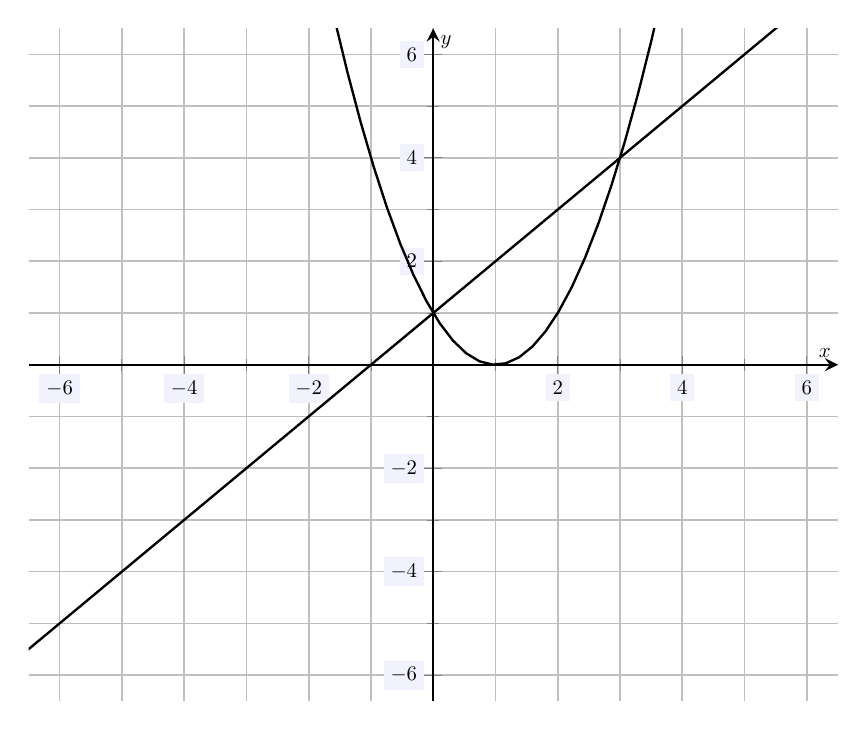
\begin{tikzpicture}[scale=1.5,every node/.style={scale=0.5}]
	\begin{axis}[
	grid=both,
	axis lines=middle,
	ticklabel style={fill=blue!5!white},
	xmin= -6.5, xmax=6.5,
	ymin= -6.5, ymax=6.5,
	xtick={-6,-4,-2,0,2,4,6},
	ytick={-6,-4,-2,0,2,4,6},
	minor tick = {-7,-6,...,7},
	xlabel=\(x\),ylabel=\(y\),
	]
	\addplot[line width= 0.02cm,samples=100,domain= -10.5:10.5] ({x},{x^2 - 2*x + 1}); 
	\addplot[line width= 0.02cm,samples=100,domain= -10.5:10.5] ({x},{x + 1}); 
	\end{axis}
	\end{tikzpicture}
	}
	\] \pspace

\begin{parts}
\part[5] Using the plot above, solve the following system of equations:
	\[
	\begin{aligned}
	-x + y&= 1 \\
	2x + y&= x^2 + 1
	\end{aligned}
	\] \pvspace{3cm}

\part[5] Setting the functions equal, verify the solution(s) to the system of equations from (a).
\end{parts}


\end{questions}
\end{document}